%cSpell:ignore Erol,Sezgin,fancyhdr, hheadheighti,hheadsepi,hfootheighti,graphicx, hfootskipi, Gavrilita, Mihail, AMOO, totalheight, keepaspectratio,UML's, kata, codewars, OOAD, COFFE,ERLANG,caml, kotlin,haskel, ruby, superclass, 
\documentclass[12pt]{article}
%\usepackage[english]{babel}
%actually it works without this package//// cuz it is in english by default... it might be useful //// but not here
% \usepackage{natbib}
% \usepackage{biblatex}

% \usepackage[backend=biber]{biblatex}

%\usepackage{url}
%idk what for it is here, it is not what it seems to be, fuck it
%%\usepackage[document]{ragged2e} 
%%to justify
% i dont use it anymore
\usepackage[utf8]{inputenc}
%%%\usepackage{amsmath}
%%useless for this report... it's for math stuff
\usepackage{graphicx}
%This package enables the user to the importation of graphics into a .tex file and, apart from the usual sizing and rotational facilities, also enables the user to crop or trim an image as desired (e.g., to get rid of surrounding blank margins). The graphicx package is useful if you need to use only a part of a complete image. 
\graphicspath{{images/}}
%% includes pics inside image folder
\usepackage{parskip}
%%this shit . In the document body, don't use \parskip but a blank line to separate paragraphs.there's normally no need to add manual line breaks (\\) in the text.

\usepackage{vmargin}
%%LaTeX package which introduces paper sizes and provides macros for setting document margins. 
\usepackage{enumerate} 
%enumeration of elements  
\usepackage{caption}
%%this is for figures
\usepackage{float}
%% to position exactly the figure 
\usepackage{fancyhdr}
%%To customize the footer and header in your document first import the package fancyhdr with 
% \addbibresource{lab4.bib}
% \bibliography{my_bibliography.bib} 
\PassOptionsToPackage{hyphens}{url}\usepackage{hyperref}
\hypersetup{
    colorlinks=true,
    linkcolor=blue,
    filecolor=magenta,      
    urlcolor=cyan,
}

\renewcommand{\theenumii}{\arabic{enumii}}
\setmarginsrb{3 cm}{2.5 cm}{3 cm}{2.5 cm}{1 cm}{1.5 cm}{1 cm}{1.5 cm}
%%\setmarginsrb{hleftmargini}{htopmargini}{hrightmargini}{hbottommargini}% {hheadheighti}{hheadsepi}{hfootheighti}{hfootskipi
\title{DB Laboratory 10}								
\author{Sezgin E}							
\makeatletter
%%The \makeatletter command temporarily defines »@« as a normal character to enable changes to internal LaTeX macros outside packages (STY) or classes (CLS).
\let\thetitle\@title
%%\let allows you to copy the content of a command into a new command.
\let\theauthor\@author
%%Thus \let\foo\bar defines \foo to have the value that \bar had at the point of definition.
\makeatother
% With \makeatother this process is reversed and the »@« is set to its original character category (other). The »@« is used to protect the internal LaTeX macros. Hence you should be very careful when using these two commands.
\pagestyle{fancy}
%%After that, the "fancy" style is set by \pagestyle{fancy}
\fancyhf{}
%%The command \fancyhf{} clears the header and footer, otherwise the elements of the default "plain" page style will appear. 
\rhead{\theauthor}
%%Prints the text included inside the braces on the right side of the header. 
\lhead{\thetitle}
%%Prints the text set inside the braces on the left side of the header.
\cfoot{\thepage}
%%\cfoot{Page \thepage}  Prints the word "Page" and next the page number which is automatically set by \thepage on the center of the footer. 
        
\begin{document}
        
        %%%%%%%%%%%%%%%%%%%%%%%%%%%%%%%%%%%%%%%%%%%%%%%%%%%%%%%%%%%%%%%%%%%%
        
        \begin{titlepage}
                \centering
                \vspace*{0.5 cm}
                
\includegraphics[scale = 0.11]{LOGO_UTM.jpg}\\[1.0 cm]	% University Logo
                %% Importing a graphic is done by using the command \includegraphics[key1=...,key2=...,etc.]{filename} Optional parameters—called “keys”—enable the figure to be resized, rotated, cropped, trimmed, etc. These keys and their functions are listed below. 
                %• scale = number — a magnification factor 
                %• width = length — the width to which the figure should be scaled1
                %• height = length — the height to which the figure should be scaled2 
                %• totalheight = length — height plus depth of figure (to be used if figure is rotated) 
                %• keepaspectratio = true/false — maintains the height/width ratio 
                %• angle = number — angle (in degrees) by which the figure is to be rotated counterclockwise 
                %• origin = location3 — the point about which rotation is to occur %• draft = true/false — prevents figure from being imported, but created a named box with the dimensions of the figure (this option is used to speed up processing) 
                %• clip = true/false — excludes whatever is outside the bounding box 
                \textsc{\LARGE Technical University of Moldova}\\[2.0 cm]%%\textsc{example text} will display the example text as small caps. All of the letters will be capitalized/uppercase, but they are going to be similar in size to a lowercase letter.	
                % University Name
                \textsc{\Large 30.11.2018}\\[0.5 cm]		% Course Code

                \rule{\linewidth}{0.2 mm} \\[0.4 cm]
                %%The \rule command in normal use produces a simple black box: \rule[raise]{width}{thickness} This is useful for drawing vertical and horizontal lines.

                { \huge \bfseries \thetitle}\\
                %%Anyway, the \bfseries bold the rest of my document, even though I'm using curly braces.
                \rule{\linewidth}{0.2 mm} \\[1.5 cm]
                
                \begin{minipage}{0.4\textwidth}
                        \begin{flushleft} \large
                                \emph{Submitted To:}\\
                                Maria Cojanu\\
                %%If you want to emphasize a word or some text, use \emph. Don't just make the text italic or bold. If needed, you may change the behavior of \emph whenever you wish in the preamble and the whole document will be adjusted accordingly.
                Asst. Univ.\\
                Computer Science Department\\
                            \end{flushleft}
                            \end{minipage}~
                            \begin{minipage}{0.4\textwidth}
                
                            \begin{flushright} \large
                            \emph{Submitted By :} \\
                            Sezgin Erol\\
                
                Group FAF-161\\
                Semester 1\\
                    \end{flushright}
                
                \end{minipage}\\[2 cm]
                
                \vfill Chisinau 2018\\  
        \end{titlepage}
        
        %%%%%%%%%%%%%%%%%%%%%%%%%%%%%%%%%%%%%%%%%%%%%%%%%%%%%%%%%%%%%%%%%%%%
        \pagebreak
        %\tableofcontents
        \subsection*{ General purpose:}
        \subsubsection*{ Learn about SQL Query Language}
        
        \subsection*{Tasks:}
        \begin{itemize}
                \item Answer Questions at the end of Chapter 10;
                \item Solve ex. 1 - 8 at the end of Chapter 10.

                
        \end{itemize}
        \subsection*{Task Realization:}
        In Figure 1 i modified existing trigger and now when any update happens in orarul table it is shown.
        \begin{figure}[H]
                \centering
                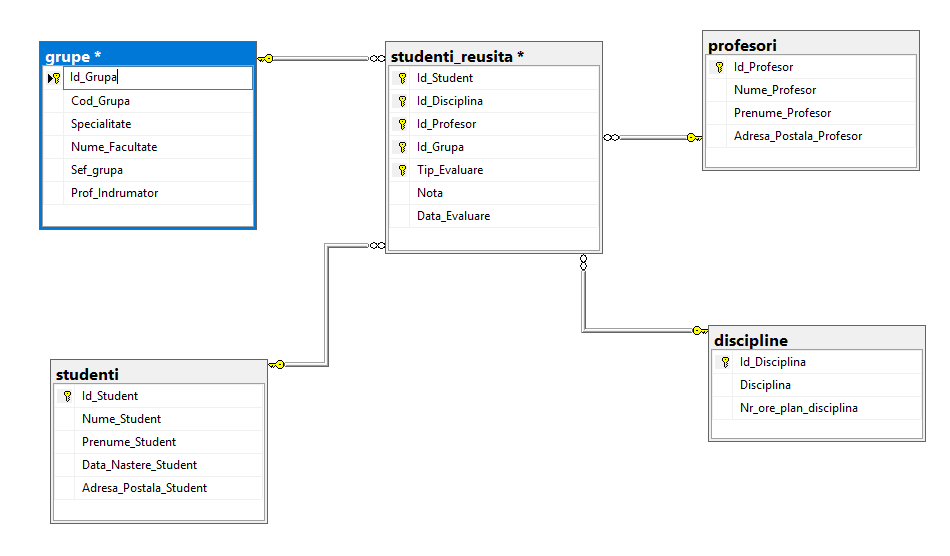
\includegraphics[width=\textwidth]{img1.png}
                \caption{Ex 1 Lab 10}
        \end{figure}
        \vspace{0.5 cm}
        
       In figure 2 I added new trigger. It process the input data to avoid any mistakes in fields.
        \begin{figure}[H]
                \centering
                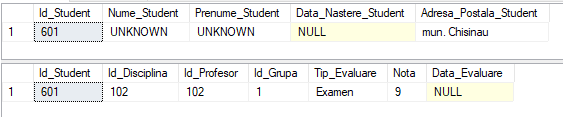
\includegraphics[width=\textwidth]{img2.png}
                \caption{Ex 2 Lab 10}
        \end{figure}
        \vspace{0.5 cm}

        In figure 3 we can observe that the error appeared because any changes are not allowed for group CIB 171 and no mark decrease is allowed.
        \begin{figure}[H]
                \centering
                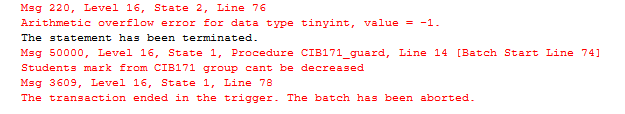
\includegraphics[width = \textwidth]{img3.png}
                \caption{Ex 3 Lab 10}
        \end{figure}
        \vspace{0.5 cm}

        In figure 4 we observe again an error message because user tries to modify  phe column idDisciplina. that is not allowed
        \begin{figure}[H]
                \centering
                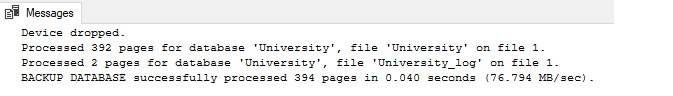
\includegraphics[width=\textwidth]{img4.png}
                \caption{Ex 4 Lab 10}
        \end{figure}
        \vspace{0.5 cm}

        In figure 5 we observe again an error message because user tries to modify the database not in work hours
        \begin{figure}[H]
                \centering
                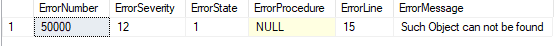
\includegraphics[width=\textwidth]{img5.png}
                \caption{Ex 5 Lab 10}
        \end{figure}
        \vspace{0.5 cm}
      
      
        
        \newpage 
        \subsection*{Conclusion}
        During This lab work i find out how to Make Triggers. They are important part of sql because they handle events, so ic case that something unexpected happens it will be cached and examined.
        \cite{SQLServerManagementStudio}
        

 
\medskip
 
\begin{thebibliography}{9}
\bibitem{SQLServerManagementStudio} 
SQL Server Management Studio 2017, Tutorials for Lab 10

\bibitem{MSSQL_} 
MSSQL Official Documentation
\url{https://docs.microsoft.com/en-us/sql/t-sql/language-elements/try-catch-transact-sql?view=sql-server-2017}
\end{thebibliography}
                
\end{document}